\documentclass[12pt,letterpaper,twocolumn]{article}
\usepackage[utf8]{inputenc}
\usepackage{graphicx} %Para importar gráficos
\usepackage[spanish, mexico]{babel} %Para que el contenido del documento esté en español de México
\usepackage[hidelinks]{hyperref} %Para el enlace al final del documento
\usepackage{amsmath}

\author{Eduardo René Rodríguez Ávila}
\title{El teorema de Pitágoras}
\begin{document}
	\maketitle
	

El teorema de Pitágoras\footnote{``En todo triángulo rectángulo el cuadrado de la hipotenusa es igual a la suma de los cuadrados de los catetos.'' Pitágoras de Salmos} establece que en todo triángulo rectángulo, el cuadrado de la hipotenusa (``el lado de mayor longitud del triángulo rectángulo'') es igual a la suma de los cuadrados de los catetos (los dos lados menores del triángulo, los que conforman el ángulo recto).

\begin{figure}[h] 
	\centering
	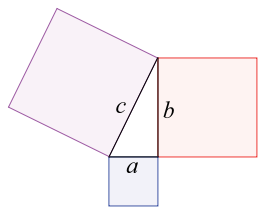
\includegraphics[width=0.4\textwidth]{img/pythagorean.png}
	\caption{Representación gráfica de los lados de un triángulo rectángulo}
\end{figure}

Si un triángulo rectángulo (ver figura 1) tiene catetos de longitudes $a$, y $b$, y la medida de la hipotenusa es $c$, se establece que:

\begin{equation}
	c^2 = a^2 + b^2
\end{equation}
  
De la ecuación 1 se deducen fácilmente 3 corolarios de aplicación práctica:

\[
a = \sqrt{c^2 - b^2} \quad  b = \sqrt{c^2-a^2} \quad  c = \sqrt{a^2 + b^2}
\]


\section{Historia}

El teorema de Pitágoras tiene este nombre porque su descubrimiento recae sobre la es\-cue\-la pitagórica. Anteriormente, en Mesopotamia y el Antiguo Egipto se conocían ternas de valores que se correspondían con los lados de un triángulo rectángulo, y se utilizaban para resolver problemas referentes a los citados triángulos, tal como se indica en algunas tablillas y papiros. Sin embargo, no ha perdurado ningún documento que exponga teóricamente su relación. La pirámide de Kefrén, datada en el siglo XXVI a. C., fue la primera gran pirámide que se construyó basándose en el llamado triángulo sagrado egipcio, de proporciones 3-4-5.

\section{Demostraciones}

El teorema de Pitágoras es de los que cuenta con un mayor número de demostraciones diferentes, utilizando métodos muy diversos. Una de las causas de esto es que en la Edad Media se exigía una nueva demostración del teorema para alcanzar el grado de "Magíster matheseos".

Algunos autores proponen hasta más de mil demostraciones. Otros autores, como el matemático estadounidense E. S. Loomis, catalogó 367 pruebas diferentes en su libro de 1927 The Pythagorean Proposition.

En ese mismo libro, Loomis clasificaría las demostraciones en cuatro grandes grupos: las algebraicas, donde se relacionan los lados y segmentos del triángulo; geométricas, en las que se realizan comparaciones de áreas; dinámicas a través de las propiedades de fuerza, masa; y las cuaterniónicas, mediante el uso de vectores.

\subsection{Demostración supuesta de Pitágoras}

Se estima que se demostró el teorema mediante semejanza de triángulos: sus lados homólogos son proporcionales.

\begin{figure}[h] 
	\centering
	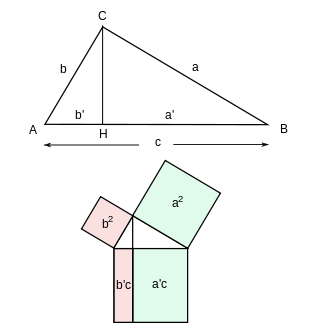
\includegraphics[width=0.4\textwidth]{img/triangulos_pitagoras.png}
	\caption{Se cree que Pitágoras se basó en la semejanza de los triángulos ABC, AHC y BHC. La figura coloreada hace evidente el cumplimiento del teorema.}
\end{figure}



Sea el triángulo ABC, rectángulo en C. El segmento CH es la altura relativa a la hipotenusa, en la que determina los segmentos $a'$ y $b'$, proyecciones en ella de los catetos $a$ y $b$, respectivamente.

Los triángulos rectángulos ABC, AHC y BHC tienen sus tres bases iguales: todos tienen dos bases en común, y los ángulos agudos son iguales bien por ser comunes, bien por tener sus lados perpendiculares. En consecuencia dichos triángulos son semejantes.

- De la semejanza entre ABC y AHC:

\begin{align*}
	    \frac{b}{b'}  & = \frac{c}{d} \\
	    b^{2} & =  b'c
\end{align*}
    
    y dos triángulos son semejantes si hay dos o más ángulos congruentes.

- De la semejanza entre ABC y BHC:

\begin{align*}
   \frac{a}{ a'} & = \frac{c}{a}\\
   a^{2} & = a'c
\end{align*}

Los resultados obtenidos son el teorema del cateto.

Sumando:
\begin{align*}
     a^2 \  + \  b^2 = a'c \ + \ b'c \  = \  c(a'+b')
\end{align*}

Pero $(a'+ b')= c$, por lo que finalmente resulta:

\[
    a^2 \ +  \ b^2 =c^2
\]
  
Mas información en: \url{http://es.wikipedia.org/wiki/Teorema_de_Pit\%C3\%A1goras}
\end{document}